\documentclass[xcolor=x11names,compress]{beamer}

%% General document %%%%%%%%%%%%%%%%%%%%%%%%%%%%%%%%%%
\usepackage{ucs}     % unicode 
\usepackage[utf8x]{inputenc}  % utf-8
\usepackage[ngerman, english]{babel}  % new german spelling 
\usepackage[T1]{tipa}
\usepackage{ragged2e}
\usepackage{graphicx}
\usepackage{tikz}
\usetikzlibrary{decorations.fractals}
\usepackage{enumitem}
\usepackage{gb4e}
\usepackage{qtree}
\usepackage{soul}
\usepackage{bbding}

%%%%%%%%%%%%%%%%%%%%%%%%%%%%%%%%%%%%%%%%%%%%%%%%%%%%%%


%% Beamer Layout %%%%%%%%%%%%%%%%%%%%%%%%%%%%%%%%%%
\useoutertheme[subsection=false,shadow]{miniframes}
\useinnertheme{default}
\usefonttheme{serif}
\usepackage{palatino}

\setbeamerfont{title like}{shape=\scshape}
\setbeamerfont{frametitle}{shape=\scshape}

\setbeamercolor*{lower separation line head}{bg=DeepSkyBlue4} 
\setbeamercolor*{normal text}{fg=black,bg=white} 
\setbeamercolor*{alerted text}{fg=red} 
\setbeamercolor*{example text}{fg=black} 
\setbeamercolor*{structure}{fg=black} 
 
\setbeamercolor*{palette tertiary}{fg=black,bg=black!10} 
\setbeamercolor*{palette quaternary}{fg=black,bg=black!10} 

\renewcommand{\(}{\begin{columns}}
\renewcommand{\)}{\end{columns}}
\newcommand{\<}[1]{\begin{column}{#1}}
\renewcommand{\>}{\end{column}}
%%%%%%%%%%%%%%%%%%%%%%%%%%%%%%%%%%%%%%%%%%%%%%%%%%


\title{Semantic Role Labeling}
\author{Arne Binder, Robert B\"arhold, Enrique Manjavacas}
\date{
	\begin{tikzpicture}[decoration=Koch curve type 2] 
		\draw[DeepSkyBlue4] decorate{ decorate{ decorate{ (0,0) -- (2,0) }}}; 
	\end{tikzpicture}  
	\\
	\vspace{0cm}
	\today
}


\begin{document}

\frame{\titlepage}

\frame{
	\frametitle{Gliederung}
	\tableofcontents
	[pausesections]
}


\section{Theoretischer Hintergrund und Motivation}
	\frame{
		\frametitle{Argumentstruktur von Verben}
		%Beispielverb - zweiseitige Argumentstruktur
	}

	\frame{
		\frametitle{thematische Rollen}
		%Abstraktion über die semantische Seite der Argumentstruktur		
	}

	\frame{
		\frametitle{Frames und Frame elements}
		%Situationsverankerte Abstraktion über die Argumentstruktur
		%Frame element gleich Rolle
		% --> target / praedikat
	}
	
	\frame{
		\frametitle{Motivation}
		%Anwendungsbeispiele 
		%Informationextraktion,...
		%Warum Rollen? theoretisches Beispiel
		%nicht aufschreiben, aber sagen - the linguists scarcity problem, zu viele daten zu wenige linguisten
	}

\section{Problemstellung}

	\frame{
		\frametitle{Problemstellung}
		\centering
		Automatische Bestimmung von Rollen
		
		\vspace{1cm} 
		%\fbox{\parbox{\dimexpr \linewidth - 2\fboxrule - 2\fboxsep}{
		\begin{center}
			\fbox{\parbox{.9\linewidth}{		
			Lassen sich semantische Rollen anhand von lexikalischen und syntaktischen Informationen eines Satzes automatisch bestimmen?
			}}
		\end{center}
		%TODO: box rum blauer Rahmen
	}

	\frame{
		\frametitle{Corpus: Salsa 2.0}
		\begin{itemize}
			\item Erstellt von der Universität Saarland %Referenz
			% weiterentwicklung des SALSA 1.0
			\item basiert auf dem TIGER-Korpus %Referenz
			\begin{itemize}
				\item Treebank über Zeitungsartikel
				\item NEGRA Tag-Set
				\item
					viele syntaktische Informationen:\\ 
					Pos-Tag, morphologische \& lemma-Informationen
			\end{itemize}
			\item enthält: ~24.000 Sätze mit 648 Prädikaten %target-word
			\item Prädikate: Nomen \& Verben
		\end{itemize}
	%	annotierung genau beschreiben (saetzengrenzen etc...)
	}	
	
	\frame{
		\frametitle{Corpus: Salsa 2.0}
		%TODO Beispielbild von Salto: kurzer Satz mit edge-labels
	}


\section{Umsetzung}
	\frame{
		\frametitle{Einschränkungen}
		\begin{figure}
		\centering
		\caption{Verteilung der Rollen}
		%TODO @enrique: bitte einfügen!
		%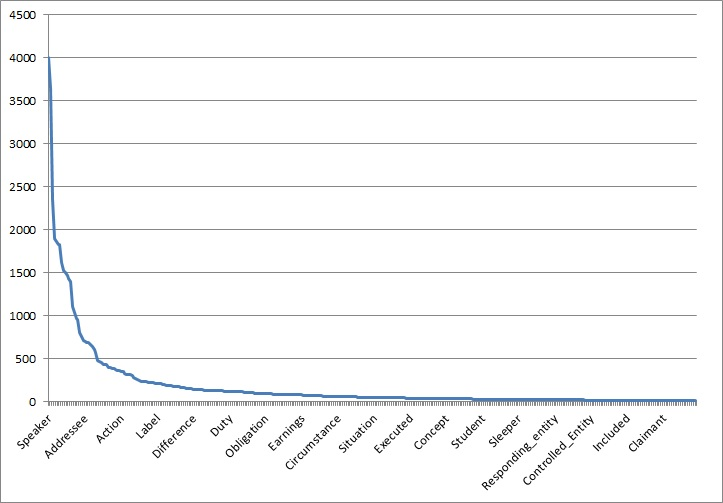
\includegraphics[scale=0.5]{images/role_frequency.jpg}
		\end{figure}
		$\Rightarrow$ Betrachtung der Top-10 Rollen		
	}
	\frame{
		\frametitle{Einschränkungen (Forts.)}
		\begin{itemize}
			\item Top-10 Rollen

			\vspace{1cm}
			\item Keine Frames
			\begin{itemize}
				\item Disambiguierung zu komplex
			\end{itemize}

			\vspace{1cm}
			\item Target-Lemma muss bekannt sein
			\begin{itemize}
				\item Keine Abstraktion für ungesehene Targets
			\end{itemize}
		\end{itemize}
	}
	
	\frame{
		\frametitle{Herangehensweise}
		\begin{itemize}
			\item Ansatz von Jurafsky und Gildea
			\begin{itemize}
				\item Classifier: Naïve Bayes Classifier
				\item Angelehnte Features
			\end{itemize}
		\end{itemize}
	}

	\frame{
		\frametitle{Prinzipieller Ablauf}
		\begin{figure}
			\caption{Training}
			%TODO @enrique: bitte einfügen!
			%\includegraphics[scale=0.5]{images/ablauf_training.jpg}
		\end{figure}
		\begin{figure}
			\caption{Klassifikation}
			%TODO @enrique: bitte einfügen!
			%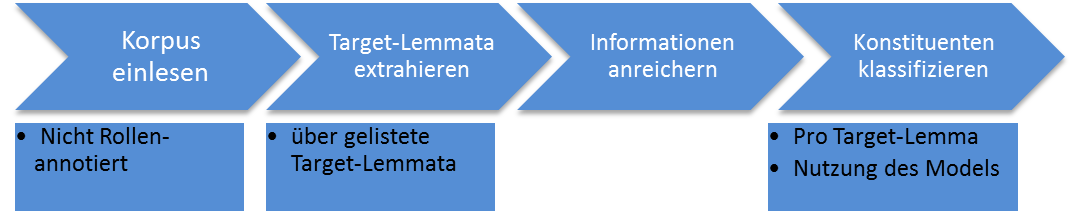
\includegraphics[scale=0.5]{images/ablauf_annotate.jpg}
		\end{figure}
		%Keine Rolle
		%smoothing: 0.000001; threshold for frame: P(R1..Rk) > e^(-600)
	}

	\frame{
 %TODO Kommentar in der E-Mail an Leser: Features einzeln mit einem Bild kurz
 % erklären statt KOmpakt + Beispiel danach
		\frametitle{Features}
		\begin{itemize}	
			\item Synt. Kategorie
			\begin{itemize}
				\item Nonterminal: phrasale Kategorie
				\item Terminal: POS-Tag
			\end{itemize}
			
			\vspace{1cm}
			\item Pfad: über synt. Kategorien
			\begin{itemize}
				\item Zusammenfassen von Replikaten 
				\item Ignorieren von Konjunktionen
			\end{itemize}

			\vspace{1cm}
			\item Position
			\begin{itemize}
				\item Position relativ zum Target
			\end{itemize}
		\end{itemize}
	}

	\frame{
		\frametitle{Features (2)}
		\begin{itemize}	
			\item Kopf-Lemma
			\begin{itemize}
				\item Syntaktisches Zentrum einer Phrase %TODO sounds strage
				\item wird regelbasiert gesucht
				%terminal =  eigenes lemma als head
			\end{itemize}

			\vspace{1cm}			
			\item Nachbar-Kopf-Lemma
			\begin{itemize}
				\item Kopf der einbettenden Konstituente
			\end{itemize}

			\vspace{1cm}
			\item Kombination: Synt. Kat. \& Pfad
		\end{itemize}
	}

	\frame{
		\frametitle{Features (3)}
		%TODO Features an Beispielsatz von Salsa-Corpus (Salto-Satz) erklären
	}

	\frame{ % ZEILENABSTAND
		\frametitle{Probleme}
		\begin{itemize}
			\item Deutsch: relativ freie Verschiebung von Konstituenten %Subjekt nicht auf die Vorfeldposition beschränkt....
			\item Kopf nicht überall definiert (NEGRA Tag-Set)

			\item Querverbindung im Syntaxgraph % KOAN BAUM
			\begin{itemize}
				\item Ich ging nach Haus' und aß Abendbrot. (Bild?)
			\end{itemize}	
					
			\item Target im Satz identifizieren
			\begin{itemize}
				\item Den Vortrag \textit{auf die lange Bank schieben.}
				\item Ich \textit{brach} den Ast \textit{ab}.
			\end{itemize}			
		\end{itemize}
	}	

\section{Evaluation}
	\frame{
		\frametitle{Evaluation}
		\begin{itemize}
			\item Target-Lemma muss vorhanden sein
			\begin{itemize}
				\item keines gefunden: Satz komplett ignoriert
			\end{itemize}
%da wir eine feste liste von target lemmata nutzen und nicht auf ungesehene targets abstrahieren koennen beruecksichtigen wird bei der evaluation nur frame elements mit dem bezug auf ein (im Model) bekanntes target. counts erklaeren und ausgeben 

			\item Nutzung des F-Mesaure
			\begin{itemize}
				\item Sehr, sehr häufig: keine Rolle % accuracy dadurch unpassend
			\end{itemize}

			\item Precision
			\begin{itemize}
				\item P = \#(Korrekte Rolle klassifiziert) / \\ \#(Klassifiziert mit Rolle)
			\end{itemize}				

			\item Recalll
			\begin{itemize}
				\item R = \#(Korrekte Rolle klassifiziert) / \\  \#(Konstituenten mit Rolle)
			\end{itemize}				
		\end{itemize}
	}

	\frame{
		\frametitle{Auswertung bezüglich dreier Kenngrößen}
		\begin{itemize} %TODO: should be enumerate
			\item Konstituente wurde korrekte Rolle zugewiesen
			\begin{itemize}
				\item Exakte Übereinstimmung
			\end{itemize}

			\item Konstituente wurde eine bel. Rolle zugewiesen
			\begin{itemize}
				\item Unabhängig von der Rolle
			\end{itemize}

			\item Korrekte Rolle wurde im Satz gefunden
			\begin{itemize}
				\item Unabhängig der Position im Satz
			\end{itemize}
		\end{itemize}
		% das letzte geht mehr auf die Rollenzählung ein, die ersten beiden sind für Konstituenten
	}

	\frame{
		%TODO Beispielsatz von Salto wieder nutzen, muss mind. 2 Rollen haben
	}


	\frame{
		\frametitle{Ergebnisse}
		\begin{itemize}
		  \item Korpus: Top-10 Rollen
		  \begin{itemize}
			  \item $\sim$ 14000 Sätzen
			  \item $\sim$ 22500 Konstituenten mit einer Rolle
		  \end{itemize}
		\end{itemize}

		\vspace{1cm}
		\begin{table}
			\small
			\caption{Ergebnisse einer 5-fach Kreuzvalidierung}
			\begin{tabular}{r|c|c|c}
			  	Typ						& Precision & Recall & F-Mesaure \\
			  	\hline
				Exaktes Match 			&  0,51 $\pm$ 0,02 & 0,81 $\pm$ 0,02 & 0,62 $\pm$ 0,02 \\
				\hline
				Unabhängig (Rolle)		&  0,67 $\pm$ 0,03 & 0,85 $\pm$ 0,02 & 0,75 $\pm$ 0,02 \\
				\hline
				Unabhängig (Position)	&  0,55 $\pm$ 0,02 & 0,88 $\pm$ 0,02 & 0,68 $\pm$ 0,02
			\end{tabular}
		\end{table}
		
		\begin{center}
			\small
			Angabe: Ergebniswert (gerundet) $\pm$ Standardabweichung
		\end{center}
	}

	\frame{
		\frametitle{Einordnung der Ergebnisse}
		\begin{itemize}
			\item Erstes SRL-Projekt auf dem SALSA 2.0 Korpus
			\vspace{1cm}

			\item Universität Saarland: Projekt auf dem SALSA 1.0 Korpus
			\begin{itemize}
				\item Prec.: 0.761  $\vert$ Recall: 0.496  $\vert$ F-Mesaure: 0.600
				\item Vorgehen \& Evaluation unklar
			\end{itemize}

			\vspace{1cm}
			\item Target-Lemma muss vorhanden sein
			\begin{itemize}
				\item 92\% der Konstituenten im Korpus ignoriert 
				%TODO  = (IDrefs overall - classified idrefs) / idrefs overall * 100
				\item $\Rightarrow$ besserer Recall $\Rightarrow$ besserer F-Measure
			\end{itemize}	
		\end{itemize}
	}

	\frame{
		\centering
		\begin{tikzpicture}[decoration=Koch curve type 2] 
			\draw[DeepSkyBlue4] decorate{ decorate{ decorate{ (0,0) -- (2,0) }}}; 
		\end{tikzpicture} \\
		\vspace{1cm}
		\begin{Large} 
			Vielen Dank für die Aufmerksamkeit! \\
			\vspace{1cm}
			Fragen?
		\end{Large}
	}

	\frame{
		\frametitle{Referenzen}
		...% TODO
	}

	\frame{
		%empty frame

	}

	\frame{
		\frametitle{Backup}

	}	








































\frame{
\frametitle{What are semantic  roles?}
\begin{itemize}
	\item<2->
			\begin{xlist}
			\ex
			\gll Peter gibt Karl Geld.\\
			\footnotesize
			\textcolor{blue}{\textit{SOURCE}}
			\footnotesize
			{}
			\footnotesize
			\textcolor{blue}{\textit{RECIPIENT} }
			\footnotesize
			\textcolor{blue}{\textit{THEMA}}
			\\
			\vspace{1cm}
	\item<3->
			
			\gll Karl bekommt Geld von Peter.\\
			\footnotesize
			\textcolor{blue}{\textit{RECIPIENT}}
			\footnotesize
			{}
			\footnotesize
			\textcolor{blue}{\textit{THEMA}}
			\footnotesize
			\textcolor{blue}{\textit{SOURCE}}
			\\
			\end{xlist}

			
\end{itemize}
}



\section[Why Semantic Roles?]{}
\frame{
\frametitle{Why Semantic Roles?}
\begin{itemize}
	\item<1-> \begin{block}{\textbf{Information Extraction}}
	\begin{itemize}
		\item "Paul hat seine Mutter get\"otet."
	\end{itemize}
	\end{block}
	\vspace{1cm}
	\item<2-> \begin{block}{\textbf{Metaphernanalyse}}
	\begin{itemize}
		\item "Paul hat seine Mutter unter die Erde gebracht."
	\end{itemize}
	\end{block}
\end{itemize}
}

\section[Our goal]{}
\frame{
\frametitle{Our goal}
\begin{itemize}
	\item<1-> Automatic Semantic Role Labeling
	\item<2-> Language: German
	\item<3-> Corpus: SALSA 2.0 (based on TIGER Corpus \& FrameNet)
	\item<4-> Framework: LingPipe 
	\vspace{1cm}
	\item<5-> \textbf{References:} C.J. Fillmore (Frame Semantics), D. Jurafsky \& D. Gildea (first implementation of a Semantic Role Labeler)
	
\end{itemize}
}



\end{document}
